\chapter{Configuration Basics}
Command Line Interface (CLI) is the preferred way to manage Vyatta. Its concepts are inspired by Juniper Networks
JunOS CLI, but commands are not the same.

Vyatta configuration is hierarchical, therefore commands to manage it are multiword, starting with operation name 
(e.g. set or delete) and ending with configuration path, like ``\texttt{set interfaces ethernet eth0 disable}''.

\begin{figure}[hc]
 \begin{center}
   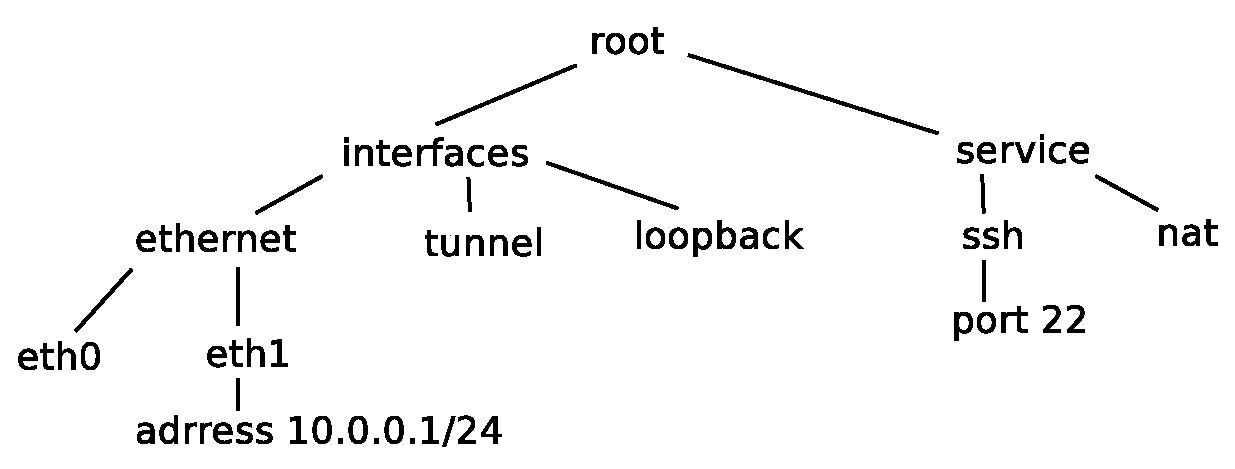
\includegraphics[width=0.5\textwidth]{images/config_tree.eps}
   \caption{Subset of Vyatta configuration tree}
  \end{center}
\end{figure}


There are two CLI modes: operational mode and configuration mode. Operational mode is what you enter right after
you logged in. It is intended for system maintenance operations, like upgrade, reboot or shutdown. You also may view
many parameters and services status from it, like DHCP leases or active VPN sessions. But you can not change system
configuration from this mode, it can be done from configuration mode only.

\section{Use operational mode}
Operational mode can be recognized by its specific command promt ending with ``\texttt{\$}''.
Like ``\texttt{vyatta@vyatta\$}''. Operational mode has various command, and they are discussed in further chapters.

\section{Enter  and exit configuration mode}
To enter configuration mode, you should issue ``\texttt{configure}'' command. Configuration mode command prompt is
different and ends with ``\texttt{\#}''. Like ``\texttt{vyatta@vyatta\#}''. To get back from configuration mode to
operational, use ``\texttt{exit}'' command.

Command set is different in operational and configuration mode, and operational commands can not be executed
``as is'' from configuration mode (and vice versa). However, there is a way not to switch between modes just to
execute an operational command.

\section{Execute an operational command from configuration mode}
Use ``\texttt{run}'' command for it. Example:
\begin{verbatim}
vyatta@vyatta# run show system uptime 
 10:34:43 up 2 days,  8:38,  2 users,  load average: 0.00, 0.00, 0.00
\end{verbatim}


\section{Execute UNIX commands}
Note that Vyatta provides full UNIX environment, and you can execute ordinary UNIX commands from CLI by just typing
them. The only thing is: there is no completion for them, completion works for Vyatta commands only. 
\texttt{\$PATH} variable also does not contain directoried like \texttt{/sbin} by default.

However, when working as an administrative user, you may use a simple workaround by executing command with
``\texttt{sudo}''. Example:
\begin{verbatim}
vyatta@vyatta:~$ sudo ls -al ~
total 28
drwxr-xr-x 1 vyatta users 4096 Nov 19 01:57 .
drwxr-xr-x 1 root   root  4096 Nov 21 08:06 ..
-rw------- 1 vyatta users 2138 Nov 21 08:08 .bash_history
-rw-r--r-- 1 vyatta users  220 Apr 10  2010 .bash_logout
-rw-r--r-- 1 vyatta users 3184 Apr 10  2010 .bashrc
-rw-r--r-- 1 vyatta users  675 Apr 10  2010 .profile
drwxr-x--- 1 vyatta users 4096 Nov 19 01:56 .ssh
\end{verbatim}
